%-------------------------------------------------------------------------------

% This file is part of Code_Saturne, a general-purpose CFD tool.
%
% Copyright (C) 1998-2011 EDF S.A.
%
% This program is free software; you can redistribute it and/or modify it under
% the terms of the GNU General Public License as published by the Free Software
% Foundation; either version 2 of the License, or (at your option) any later
% version.
%
% This program is distributed in the hope that it will be useful, but WITHOUT
% ANY WARRANTY; without even the implied warranty of MERCHANTABILITY or FITNESS
% FOR A PARTICULAR PURPOSE.  See the GNU General Public License for more
% details.
%
% You should have received a copy of the GNU General Public License along with
% this program; if not, write to the Free Software Foundation, Inc., 51 Franklin
% Street, Fifth Floor, Boston, MA 02110-1301, USA.

%-------------------------------------------------------------------------------

\section{Solution for case6}

$\bullet$ {\bf Step 1}: check the post-install required for coupling \CS with \syrthes.\\
The first step is to check the post-install required for coupling with \syrthes and verify
if the \syrthes \texttt{PATH} is correctly known in the system environment. We just need to
edit the batch file\footnote{see the installation guide, name \texttt{install.pdf}, in
\texttt{<install-prefix>/share/doc/code\_saturne/} directory.} name \texttt{code\_saturne.cfg}
as below: \\
\fbox{\begin{minipage}{\textwidth}\texttt{                       \\
\$ {\color{blue} vim <install-prefix>/etc/code\_saturne.cfg}      \\
>\#\#\# Set the location to the \syrthes installation directory. \\
> syrthes = <install-prefix-syrthes>
}\end{minipage} }

$\bullet$ {\bf Step 2}: source the \texttt{syrthes.profile} file in your user environment.\\
Before using \syrthes alone, you have to copy and source this file to define \syrthes environment
variables (like \texttt{\$SYRTHES4\_HOME}) in your terminal, as follows:\\
\fbox{\begin{minipage}{\textwidth}\texttt{                                \\
\$ {\color{blue} cp <install-prefix-syrthes>/bin/syrthes.profile .}        \\
\$ {\color{blue} source syrthes.profile}                                   \\
\$ echo \$SYRTHES4\_HOME (to check the \syrthes PATH in your environment)
}\end{minipage} }
After having defined correctly your environment, to be able to launch a coupling computation
\CS-\syrthes or a \syrthes computation alone, you just have to create the coupling study directory.

$\bullet$ {\bf Step 3}: create the \texttt{3disks2D} study directory, two subdirectories
\texttt{fluid} and \texttt{solid}.

This is done using the standard command:\\
\fbox{\begin{minipage}{\textwidth}\texttt{                                \\
\$ {\color{blue} code\_saturne create -s 3disks2D -c fluid --syrthes solid}\\
> code\_saturne 3.0 study/case generation                                 \\
> o Creating study '3disk2D' ...                                          \\
> o Creating case 'fluid' ...                                             \\
> SYRTHES4 home directory: <install-prefix-syrthes>                       \\
> MPI home directory:   /usr                                              \\
>                                                                         \\
>**************************************************                       \\
> solid : creating SYRTHES case ...                                       \\
> <install-prefix-syrthes>                                                \\
> OK !                                                                    \\
>**************************************************
}\end{minipage} }

$\bullet$ {\bf Remark}: The fluid mesh must be copied in the directory \texttt{MESH}.
The solid mesh must be copied in the subdirectory \texttt{solid}.
\newpage

\subsection{Launching the SYRTHES computation alone}

The preparation of the computation for \texttt{case5} is defined below:                                \\
\fbox{\begin{minipage}{\textwidth}\texttt{                                                             \\
$\bullet$ {\bf Step 1}: launch the \syrthes Graphical USer Interface (\texttt{syrthes.gui}),           \\
$\bullet$ {\bf Step 2}: open a {\bf New Data File},                                                    \\
$\bullet$ {\bf Step 3}: check the name of the mesh and convert this one in \texttt{.syr} format,       \\
$\bullet$ {\bf Step 4}: define the initial and boundary conditions for the conduction problem, \\
$\bullet$ {\bf Step 5}: define the physical properties of each disk \{1, 2, 3 and 4\},                 \\
$\bullet$ {\bf Step 6}: running the \syrthes computation alone.
}\end{minipage} }

$\bullet$ {\bf Step 1}: launch the \syrthes Graphical User Interface (Gui).\\
The \syrthes Graphical User Interface is launched by the following command lines in the solid subdirectory:\\
\fbox{\begin{minipage}{\textwidth}\texttt{                                                             \\
\$ cd 3disks2D/solid/                                                                                  \\
\$ {\color{blue}syrthes.gui \&}
}\end{minipage} }

$\bullet$ {\bf Step 2}: choose a New Data File inside the (Gui). \\
%In the item {\itshape Initialization} under the heading {\itshape Volume conditions}, set the initial value of the temperature
%in the domain to 20.0\degresC.
\begin{figure}[h!]
\begin{center}
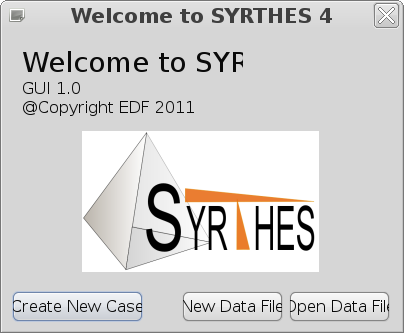
\includegraphics[width=12cm]{case6_solid_V-1}
\caption{Running the SYRTHES's IHM with syrthes.gui}
\label{fig1_e5}
\end{center}
\end{figure}
%[0]
\newpage

\begin{figure}[h!]
\begin{center}
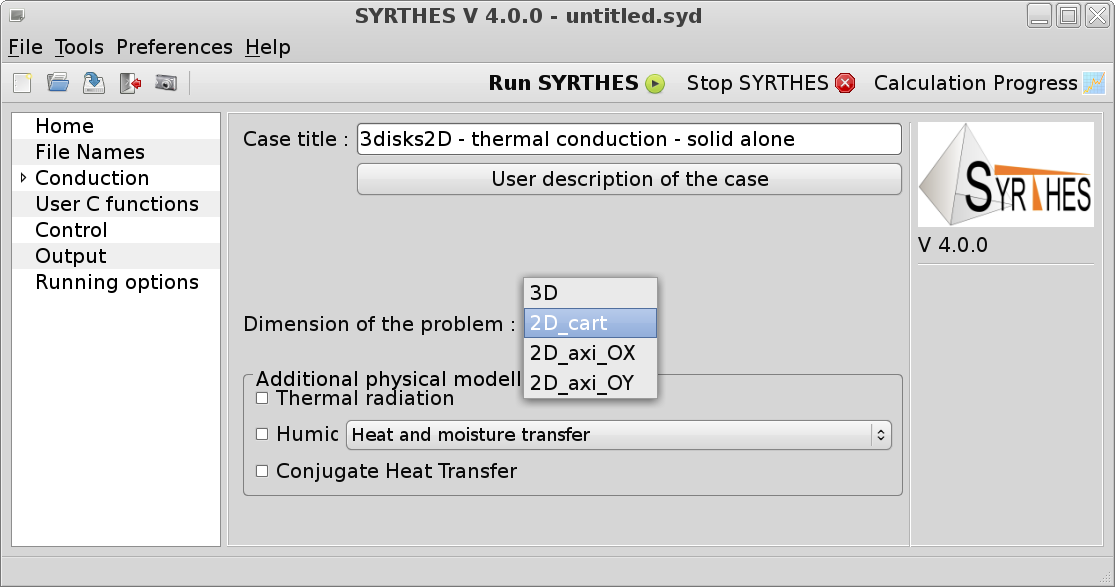
\includegraphics[width=12cm]{case6_solid_V-2}
\caption{Define the dimension and physical modelling of the problem treated}
\label{fig1_e5}
\end{center}
\end{figure}

\begin{figure}[h!]
\begin{center}
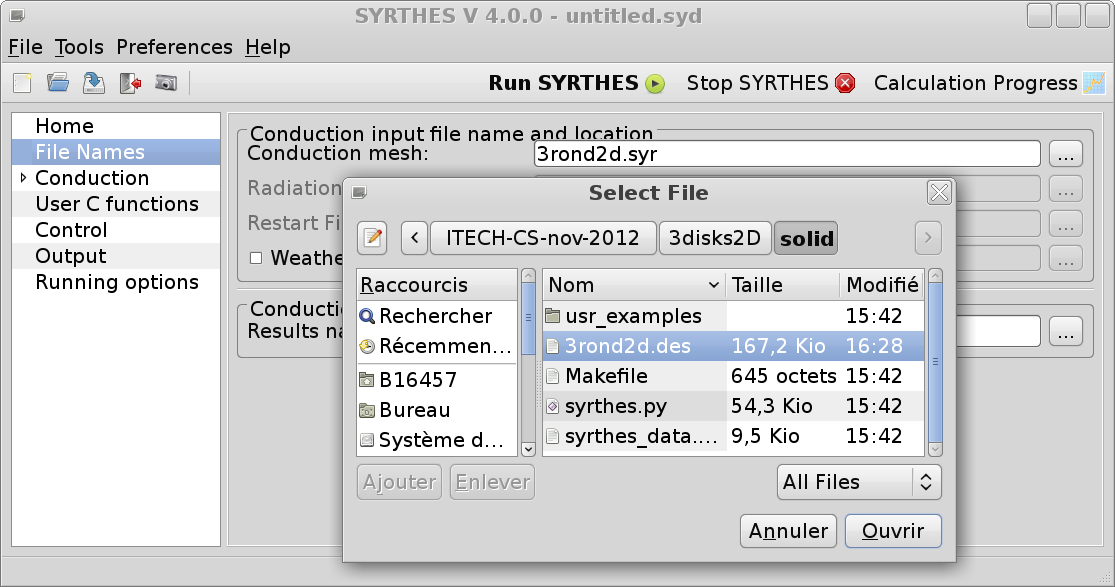
\includegraphics[width=12cm]{case6_solid_V-3}
\caption{Choose the 2D solid mesh file with the format \texttt{.des}.}
\label{fig1_e5}
\end{center}
\end{figure}
%[1]
\newpage

\begin{figure}[h!]
\begin{center}
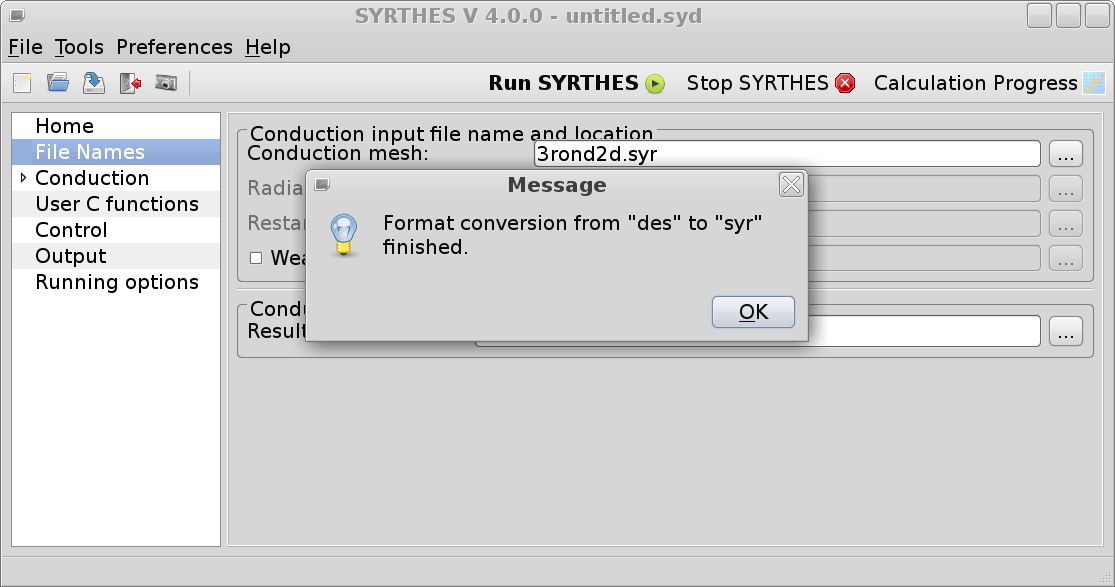
\includegraphics[width=12cm]{case6_solid_V-4}
\caption{The \syrthes (Gui) directly converts the \texttt{.des} to the \texttt{.syr} format.}
\label{fig1_e5}
\end{center}
\end{figure}

$\bullet$ {\bf Remark}: Inside the \syrthes Graphical USer Interface (Gui), we can load the \simail
format \texttt{*.des} for the solid mesh. This one will be automatically transformed to the \texttt{*.syr} format.\\
It can also be done with the following command line:\\
\fbox{\begin{minipage}{\textwidth}\texttt{                                                             \\
\$ {\color{blue}convert2syrthes4 -m 3rond2d.des}
}\end{minipage} }

$\bullet$ {\bf Remark}: You can convert the \texttt{*.syr} format into a \texttt{*.med} format.
Like that, you can load the \texttt{*.med} file inside \salome, after having used this command line below:\\
\fbox{\begin{minipage}{\textwidth}\texttt{                                                             \\
\$ {\color{blue}syrthes4med30 -m 3rond2d.syr -o 3rond2d.med}
}\end{minipage} }

\begin{figure}[h!]
\begin{center}
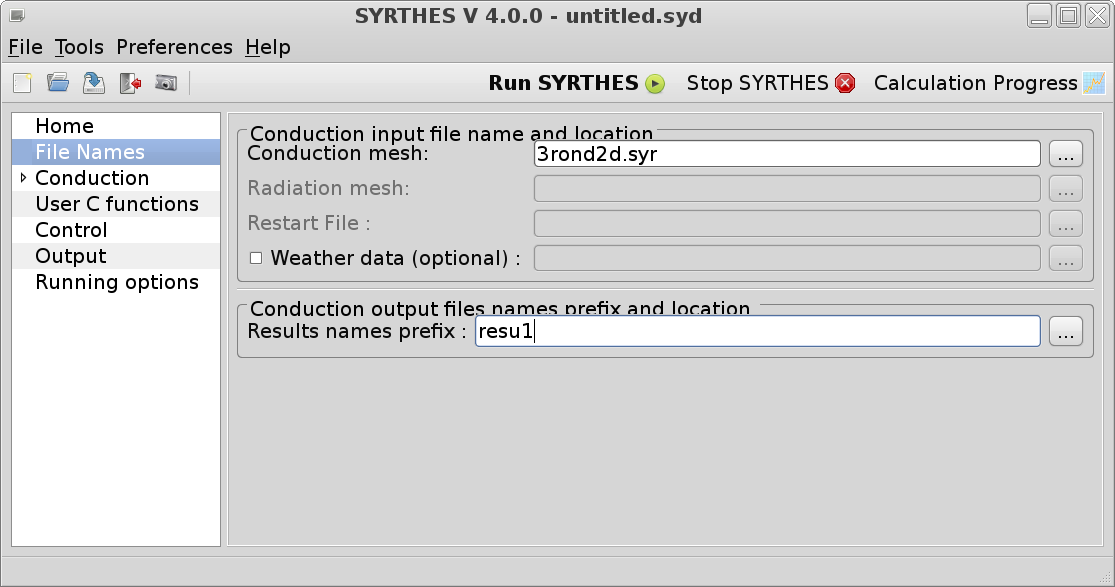
\includegraphics[width=12cm]{case6_solid_V-5}
\caption{Choose a name for the results files \texttt{.res}, \texttt{.his} and \texttt{.rdt}}
\label{fig1_e5}
\end{center}
\end{figure}
%[2]
\newpage

\begin{figure}[h!]
\begin{center}
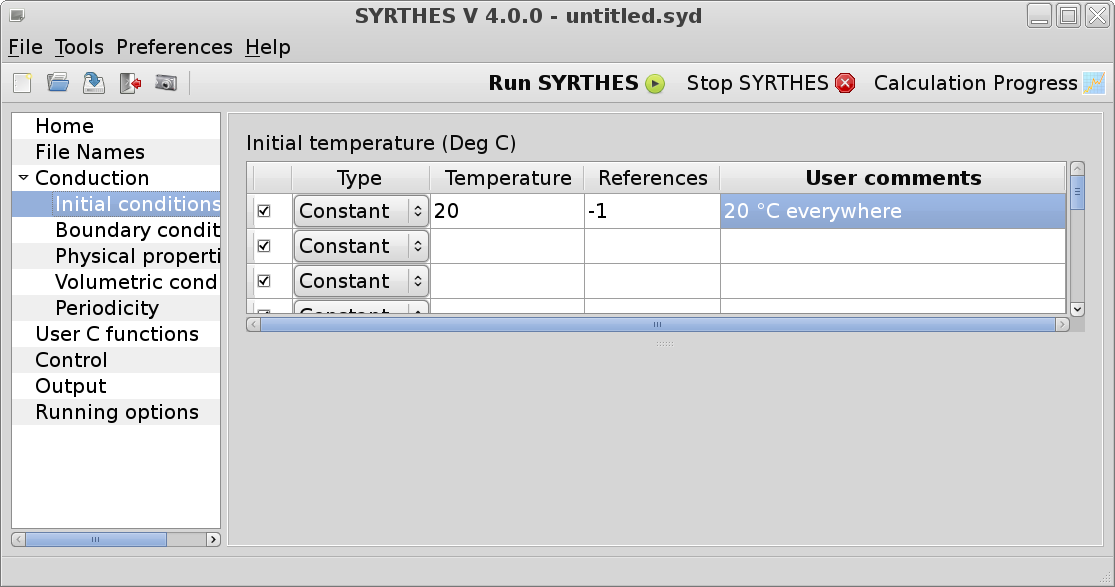
\includegraphics[width=12cm]{case6_solid_V-6}
\caption{Define the initial temperature conditions inside the different disks.}
\label{fig1_e5}
\end{center}
\end{figure}

\begin{figure}[h!]
\begin{center}
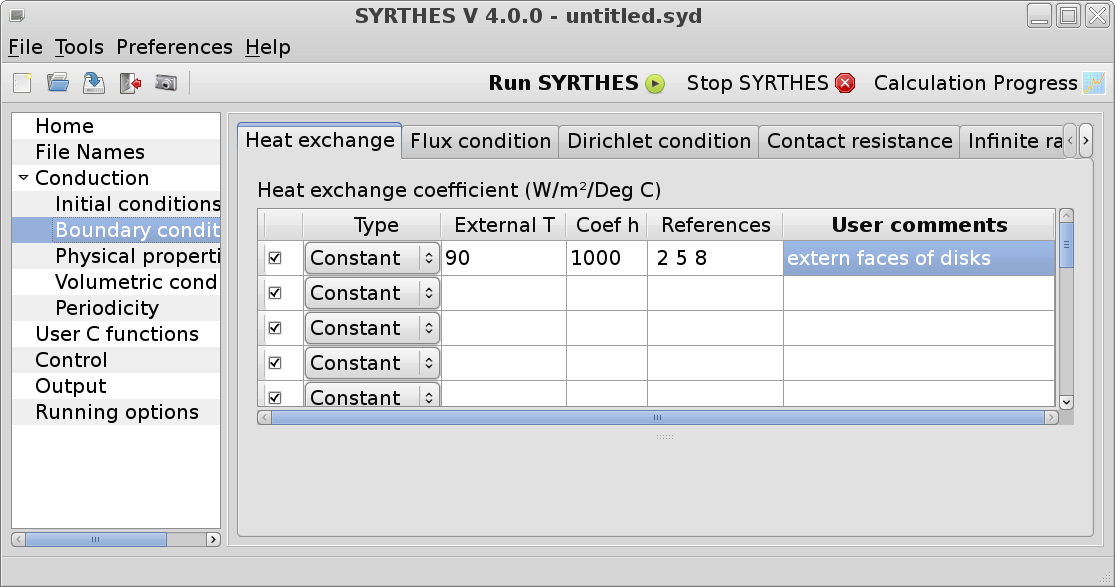
\includegraphics[width=12cm]{case6_solid_V-7}
\caption{Define the temperature boundary conditions for the extern face of the three disks.}
\label{fig1_e5}
\end{center}
\end{figure}
%[3]
\newpage

\begin{figure}[h!]
\begin{center}
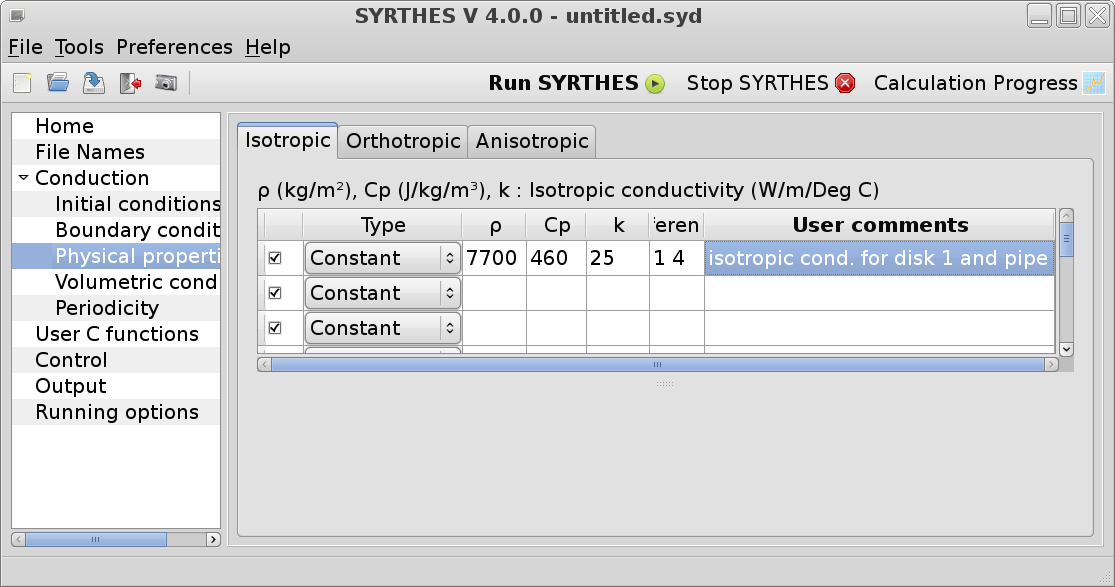
\includegraphics[width=12cm]{case6_solid_V-8}
\caption{Define the physical properties for the disk 1 and 4 with isotropic conductivity.}
\label{fig1_e5}
\end{center}
\end{figure}

\begin{figure}[h!]
\begin{center}
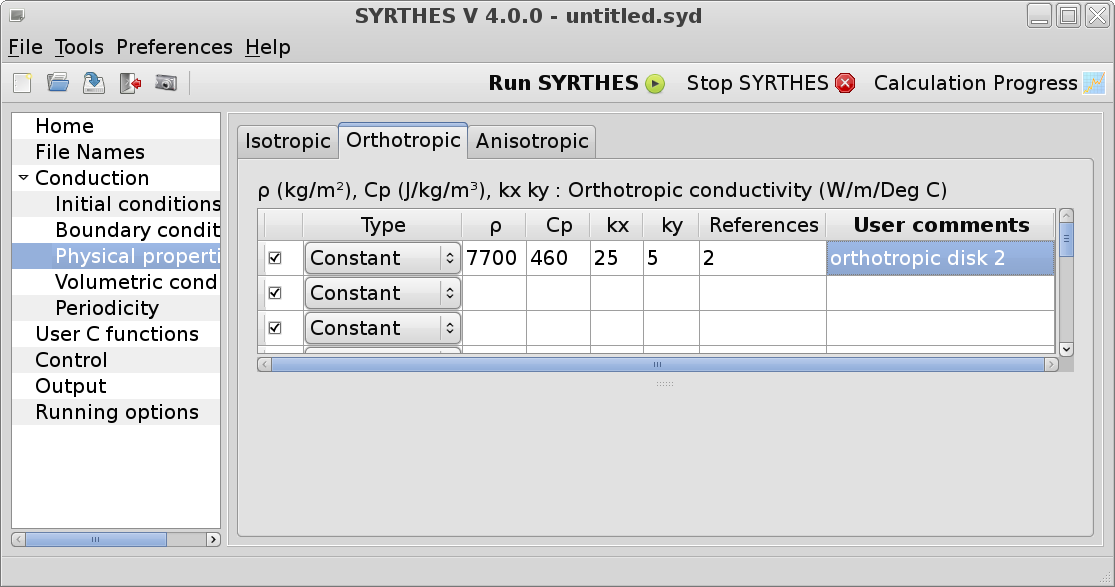
\includegraphics[width=12cm]{case6_solid_V-9}
\caption{Define the physical properties for the disk 2 with isotropic conductivity.}
\label{fig1_e5}
\end{center}
\end{figure}
$\bullet$ {\bf Remark}: To correctly identify the volume references associated to
a specific physical property, we can check the mesh regions directly inside ParaView after
having used following command line: \\
\fbox{\begin{minipage}{\textwidth}\texttt{                                                      \\
\$ {\color{blue}syrthes4ensight -m 3rond2d.syr -o mesh\_3rond2d}                                \\
******************************************************                                          \\
--> geometry file name : mesh\_3rond2d.ensight.geom                                             \\
--> case file name : mesh\_3rond2d.ensight.case
}\end{minipage} }
%[4]
\newpage

\begin{figure}[h!]
\begin{center}
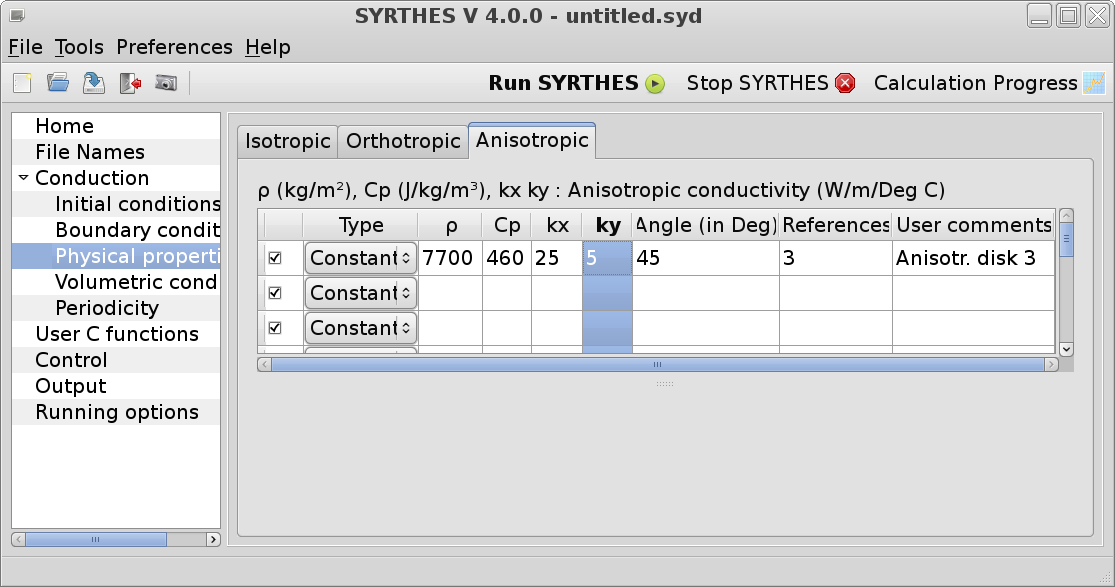
\includegraphics[width=12cm]{case6_solid_V-10}
\caption{Define the Physical properties for the disk 3 with anisotropic conductivity.}
\label{fig1_e5}
\end{center}
\end{figure}

\begin{figure}[h!]
\begin{center}
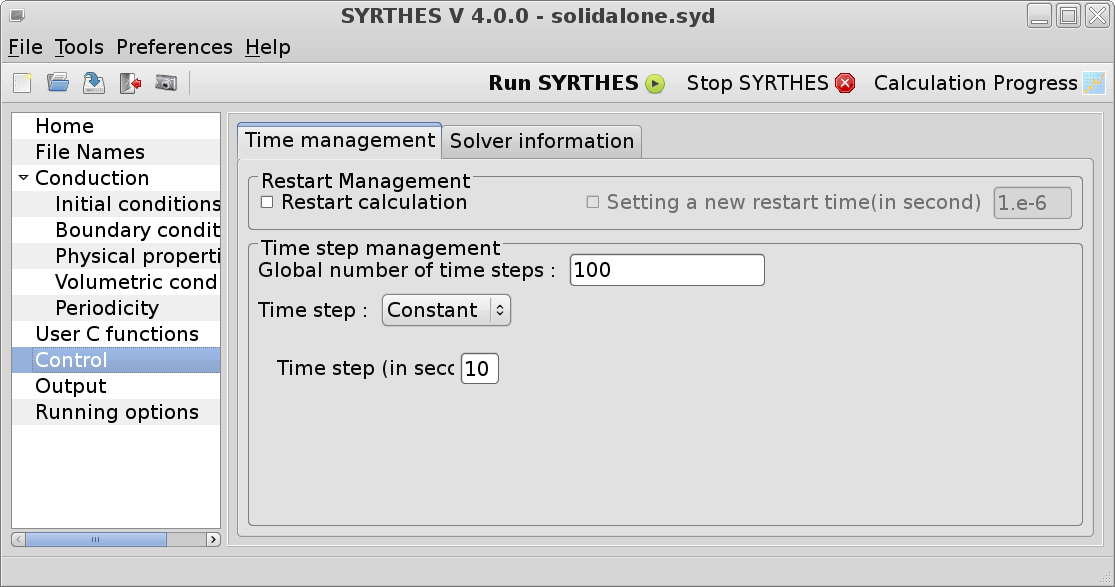
\includegraphics[width=12cm]{case6_solid_V-11}
\caption{Define the global number of time steps and the time step for the 2D solid conduction computation.}
\label{fig1_e5}
\end{center}
\end{figure}
%[5]
\newpage

\begin{figure}[h!]
\begin{center}
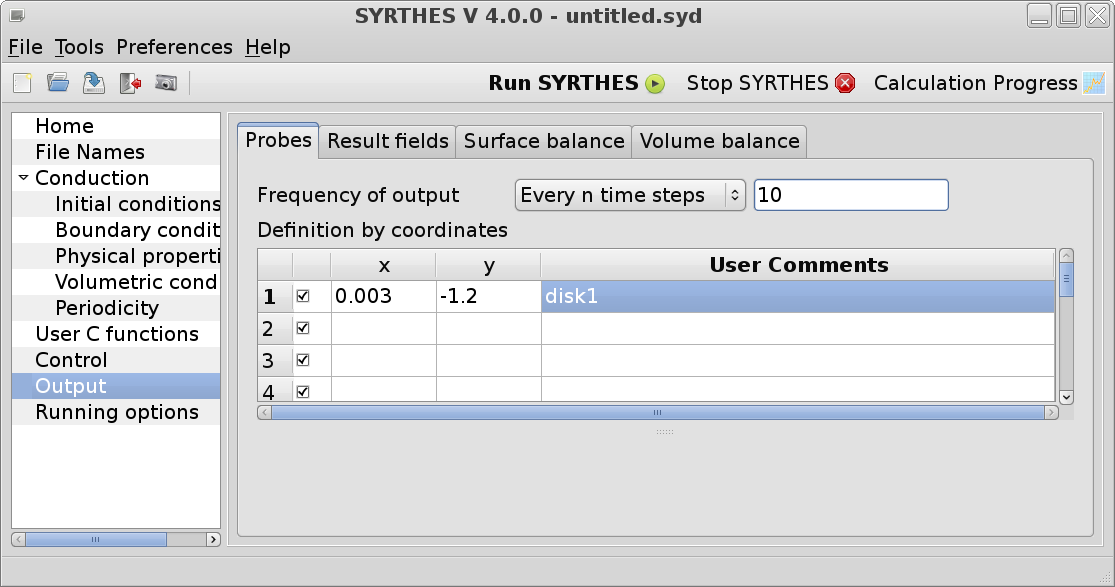
\includegraphics[width=12cm]{case6_solid_V-12}
\caption{Define the probe coordinates for output management.}
\label{fig1_e5}
\end{center}
\end{figure}

\begin{figure}[h!]
\begin{center}
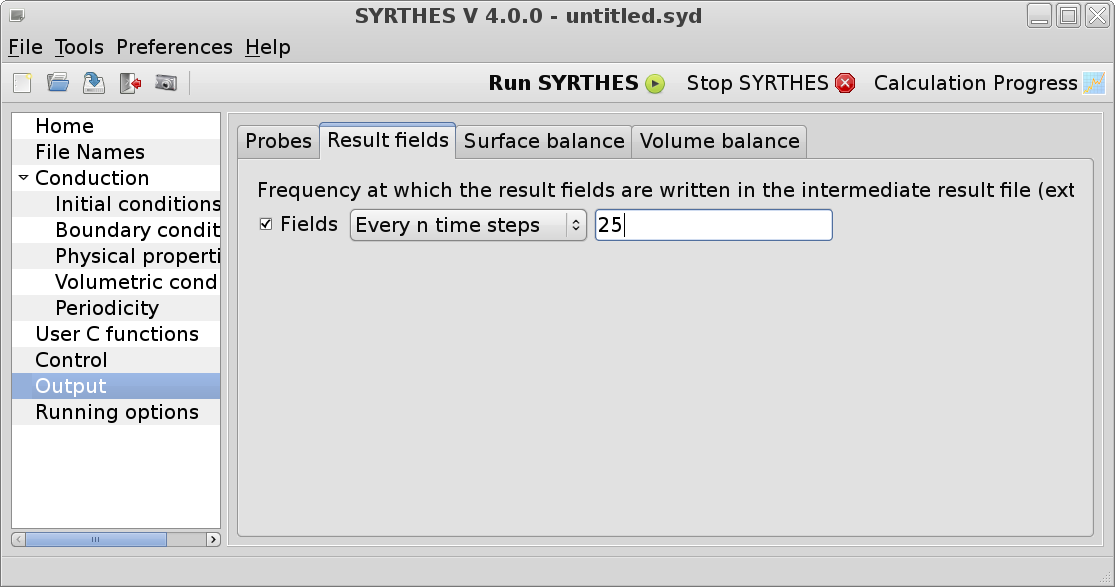
\includegraphics[width=12cm]{case6_solid_V-13}
\caption{Define the frequency at which the results fields are written}
\label{fig1_e5}
\end{center}
\end{figure}
%[6]
\newpage

\begin{figure}[h!]
\begin{center}
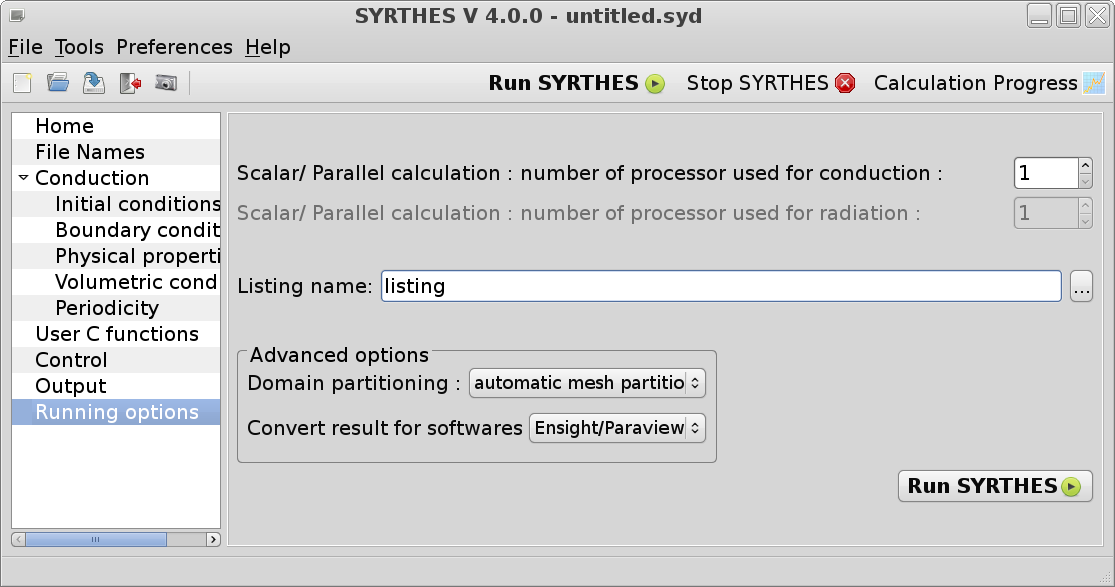
\includegraphics[width=12cm]{case6_solid_V-14}
\caption{Define the file name of the SYRTHES listing and the number of processors used.}
\label{fig1_e5}
\end{center}
\end{figure}

\begin{figure}[h!]
\begin{center}
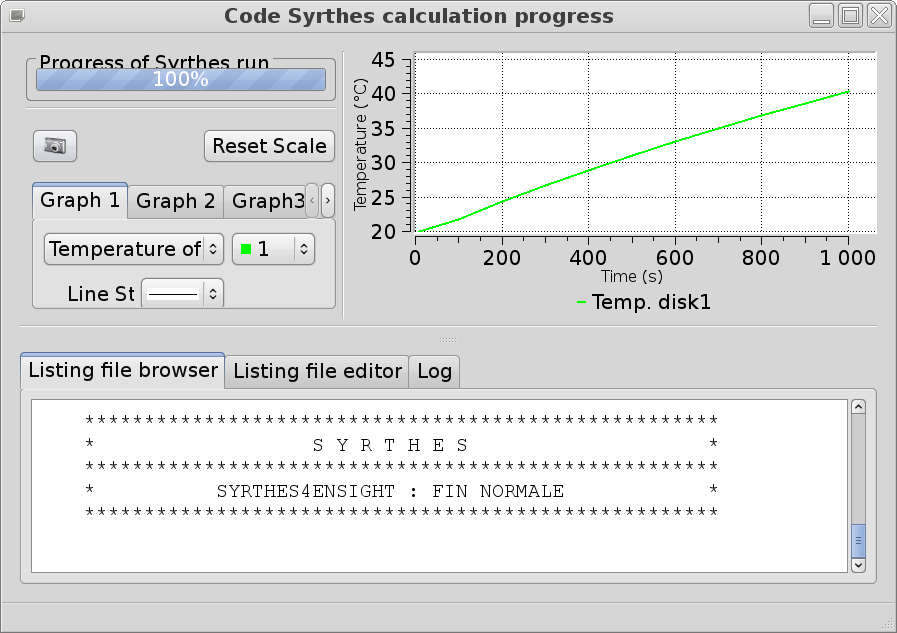
\includegraphics[width=12cm]{case6_solid_V-15}
\caption{Screenshot of the computation progress window.}
\label{fig1_e5}
\end{center}
\end{figure}
%[7]
\newpage

\begin{figure}[h!]
\begin{center}
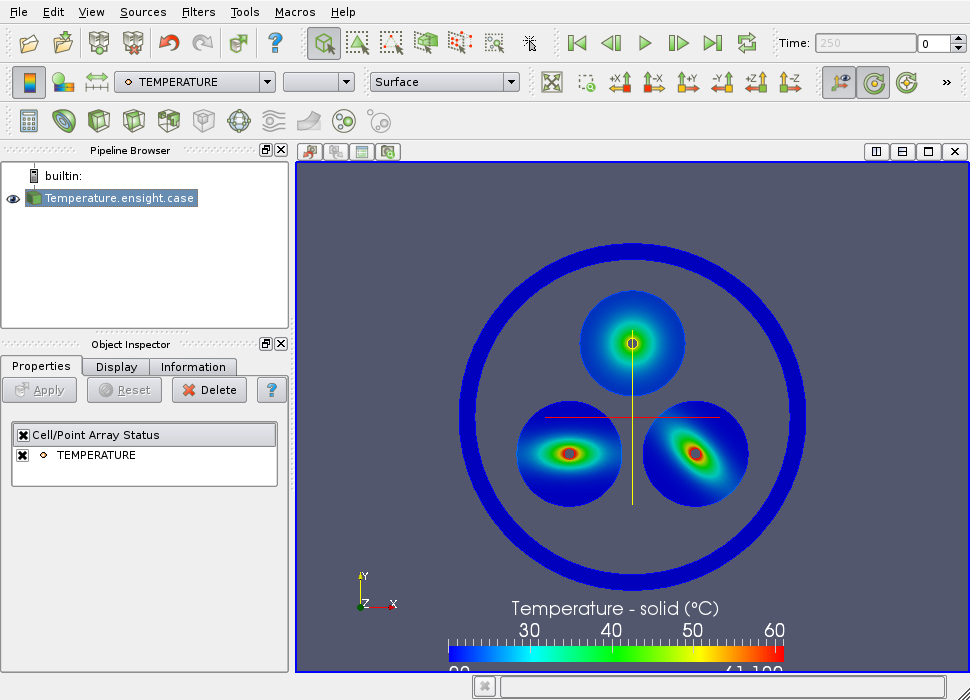
\includegraphics[width=12cm]{case6_visu_solid-00}
\caption{Screenshot of the 2D solid temperature Field.}
\label{fig1_e5}
\end{center}
\end{figure}

$\bullet$ {\bf Remark}: We can visualize the temperature results fields by applying the following command line
to the results file \texttt{resu1.res} or \texttt{resu1.rdt} (for the results saved at the last time step or the
results saved at each time step):                                   \\
\fbox{\begin{minipage}{\textwidth}\texttt{                          \\
\$ {\color{blue} syrthes4ensight -m 3rond2d.syr -r resu1.res -o Results\_Temp}   \\
\$ {\color{blue} syrthes4ensight -m 3rond2d.syr -r resu1.rdt -o Chrono\_Temp }
}\end{minipage} }
%[8]
\newpage

\subsection{Launching the \CS computation alone}

The preparation of the fluid computation alone for \texttt{case5} is defined below:\\
$\bullet$ {\bf Step 1}: launch the \CS Graphical User Interface (\texttt{./SaturneGUI}),           \\
$\bullet$ {\bf Step 2}: open a {\bf New case},                                                     \\
$\bullet$ {\bf Step 3}: check the quality of the fluid mesh with the \texttt{check\_mesh},         \\
$\bullet$ {\bf Step 4}: define the initial and boundary conditions for the air flow problem,       \\
$\bullet$ {\bf Step 5}: define the physical properties of the disk for the air flow,               \\
$\bullet$ {\bf Step 6}: running the \CS computation alone.                                         \\

\begin{figure}[h!]
\begin{center}
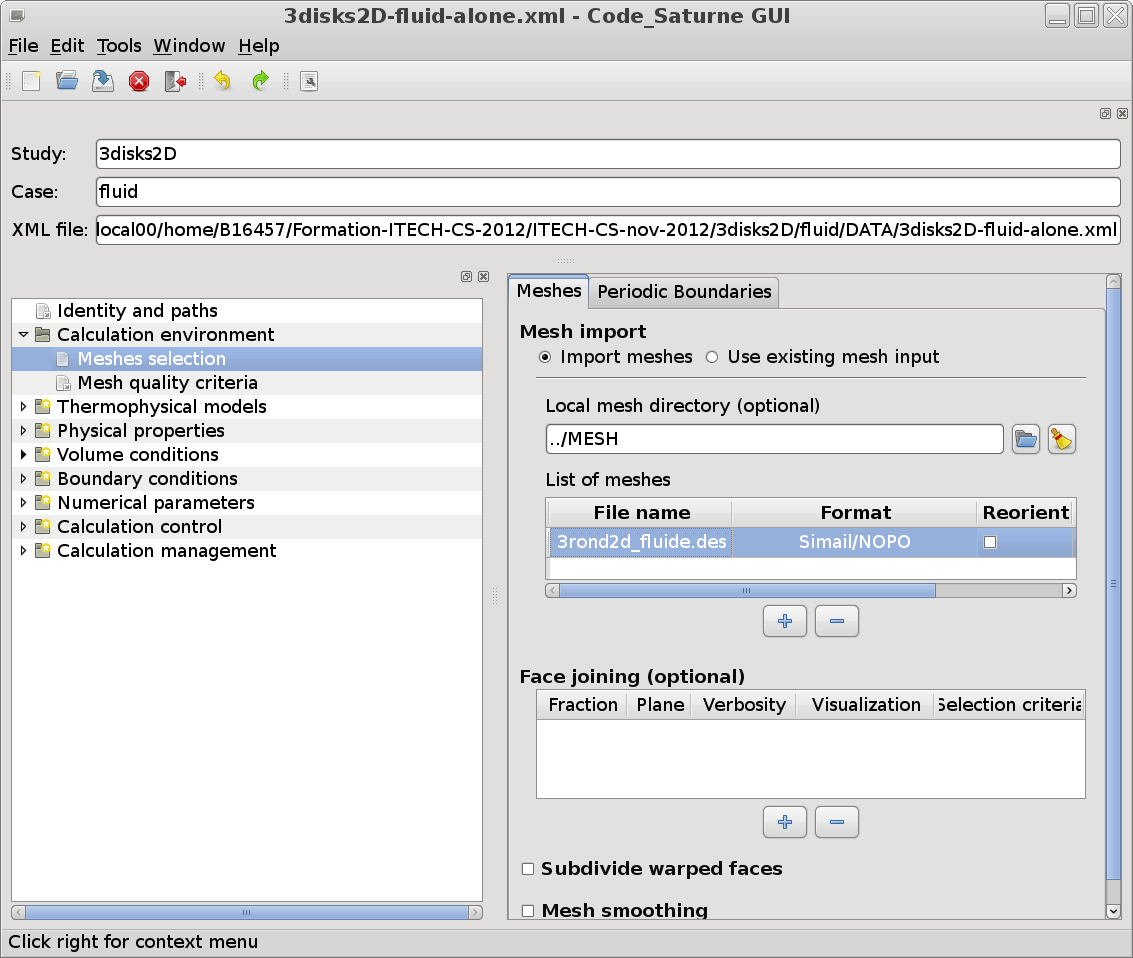
\includegraphics[width=12cm]{case6_fluid_V-1}
\caption{Choose the fluid mesh with \CS (GUI)}
\label{fig1_e5}
\end{center}
\end{figure}
%[1]
\newpage

\begin{figure}[h!]
\begin{center}
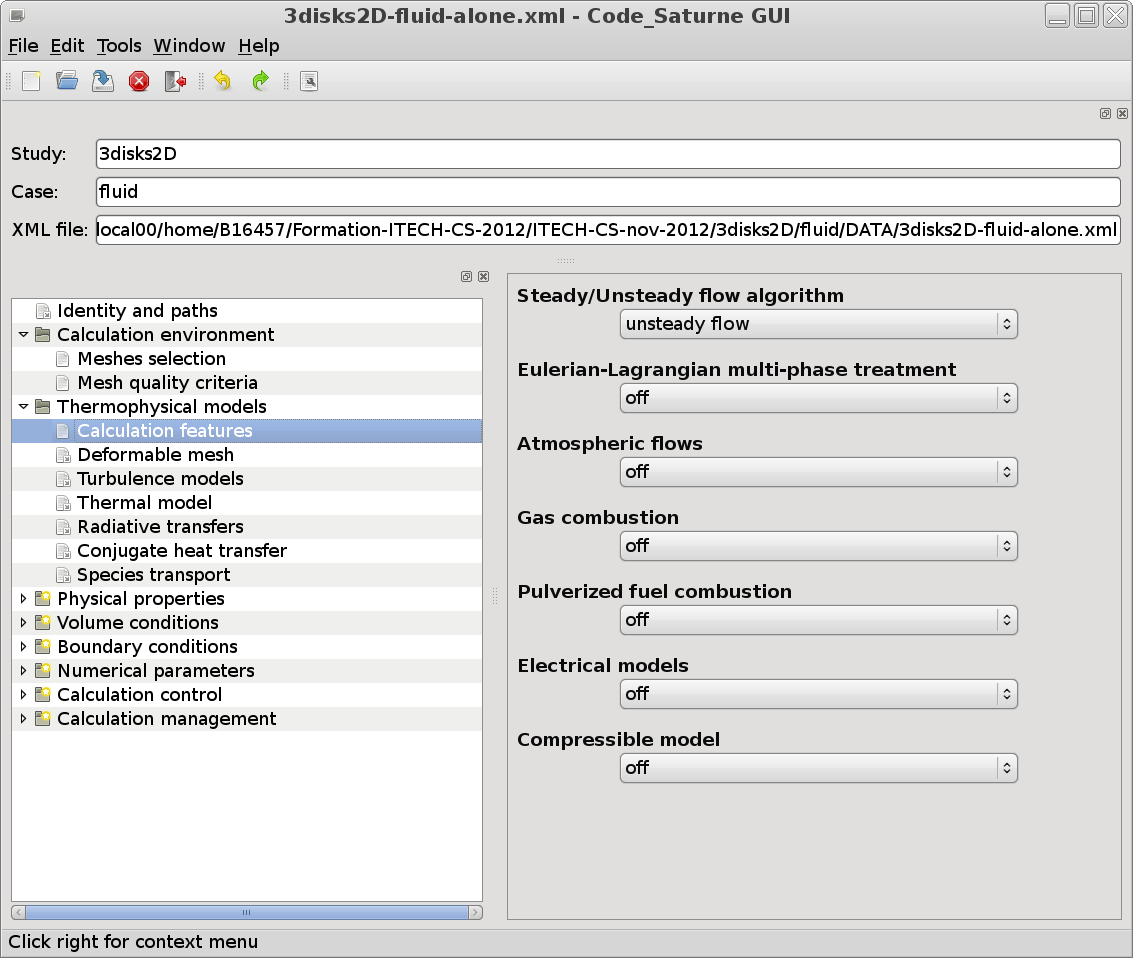
\includegraphics[width=9cm]{case6_fluid_V-2}
\caption{Define the physical modelling associated to the air flow inside the fluid domain.}
\label{fig1_e5}
\end{center}
\end{figure}

\begin{figure}[h!]
\begin{center}
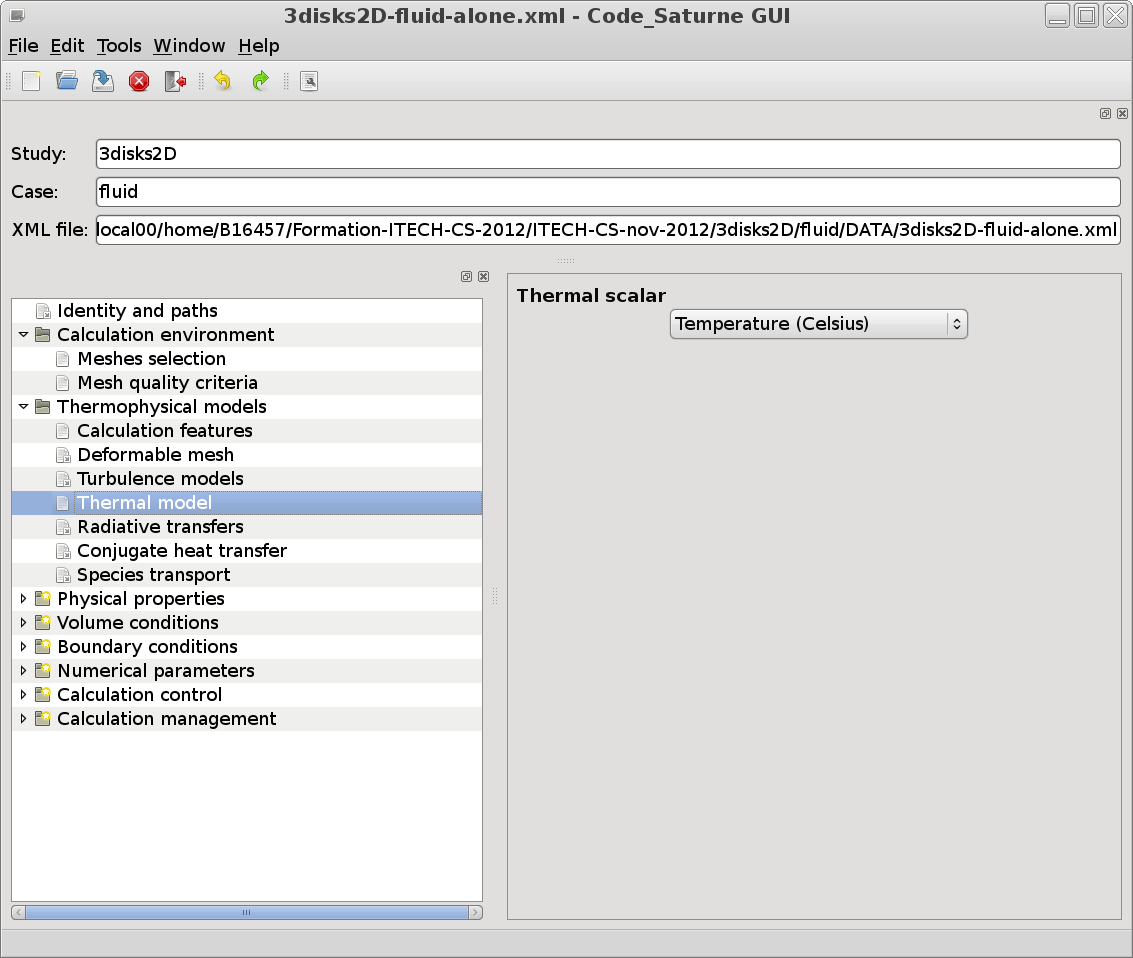
\includegraphics[width=9cm]{case6_fluid_V-3}
\caption{Choose the Temperature scalar.}
\label{fig1_e5}
\end{center}
\end{figure}
%[2]
\newpage

\begin{figure}[h!]
\begin{center}
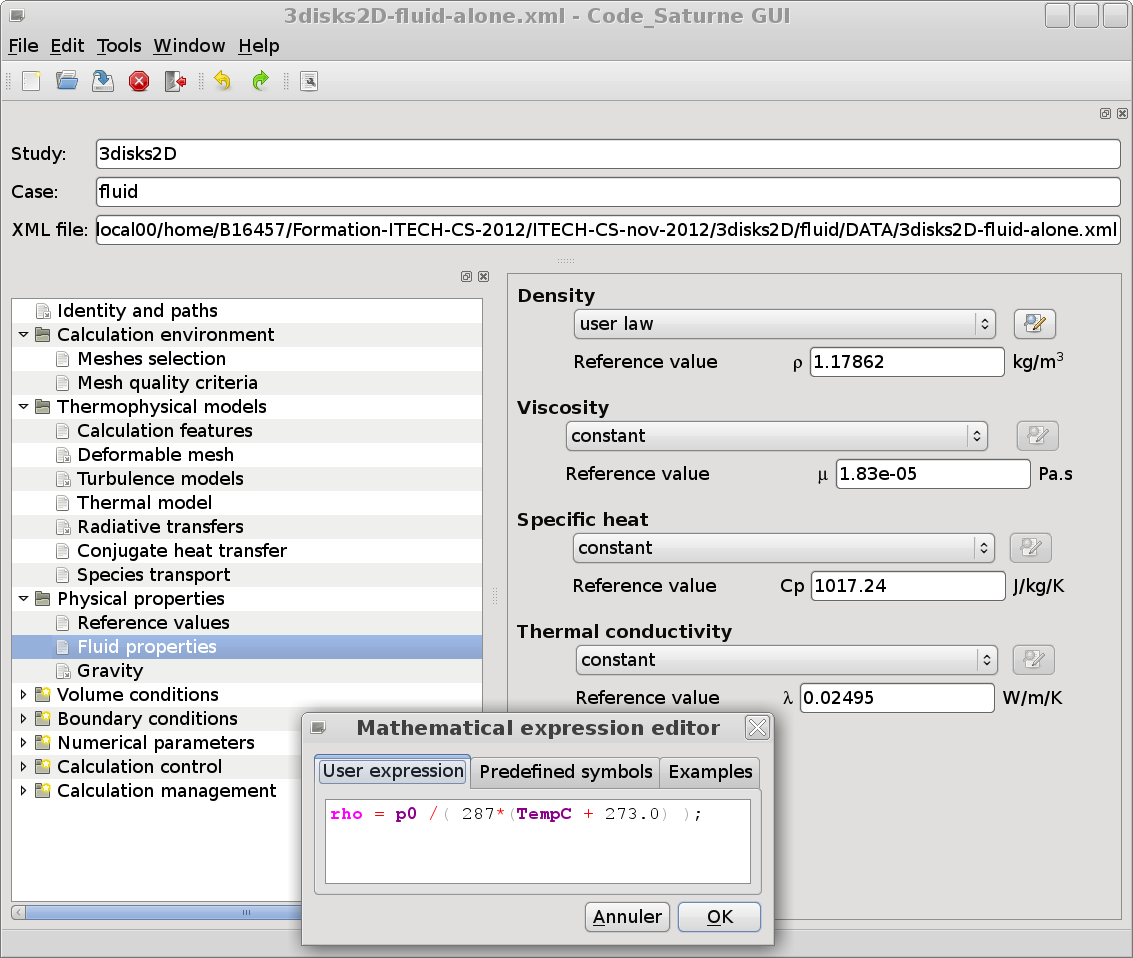
\includegraphics[width=9cm]{case6_fluid_V-4}
\caption{Define the variable density with a ideal gas law inside the \CS (GUI).}
\label{fig1_e5}
\end{center}
\end{figure}

\begin{figure}[h!]
\begin{center}
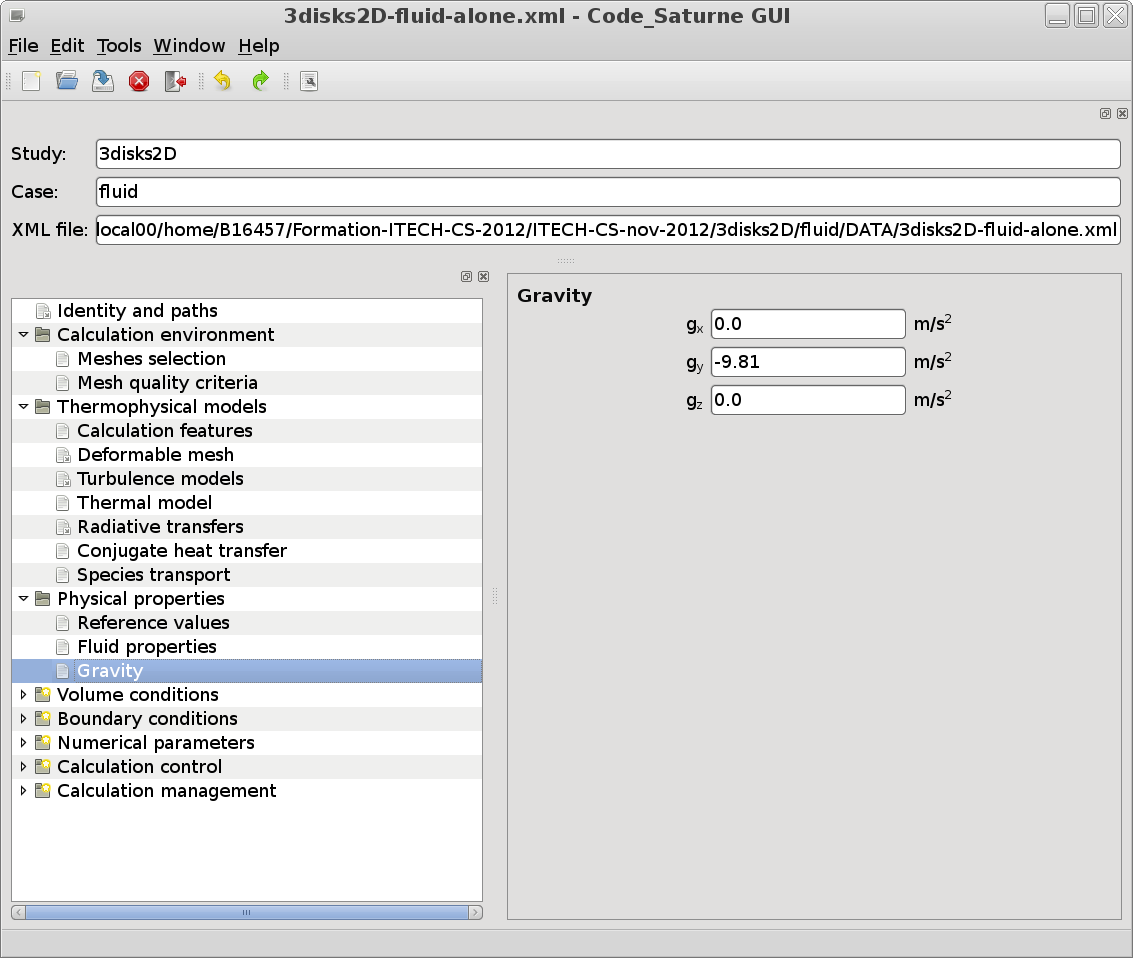
\includegraphics[width=9cm]{case6_fluid_V-5}
\caption{Define the gravity}
\label{fig1_e5}
\end{center}
\end{figure}
%[3]
\newpage

\begin{figure}[h!]
\begin{center}
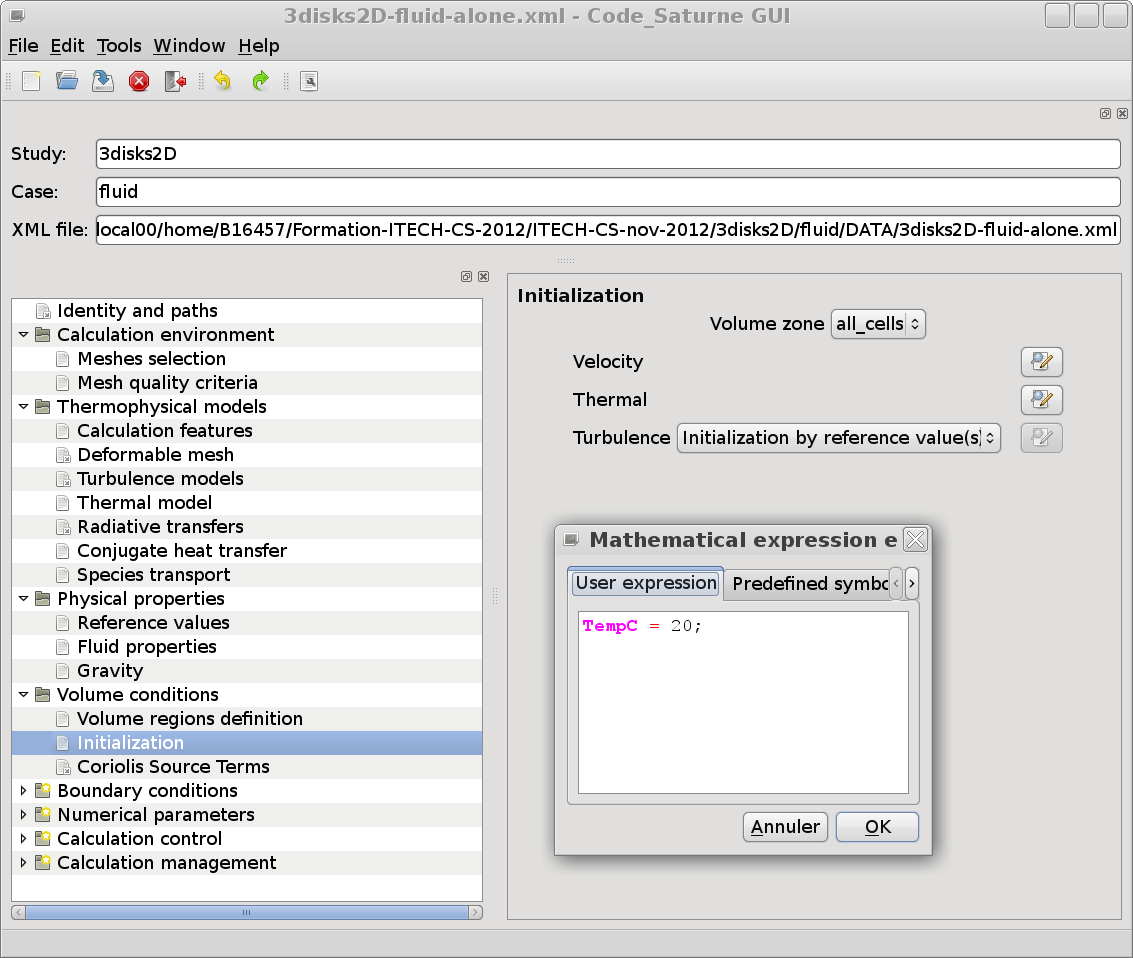
\includegraphics[width=9cm]{case6_fluid_V-6}
\caption{Initalization of the velocity components and temperature variables.}
\label{fig1_e5}
\end{center}
\end{figure}

\begin{figure}[h!]
\begin{center}
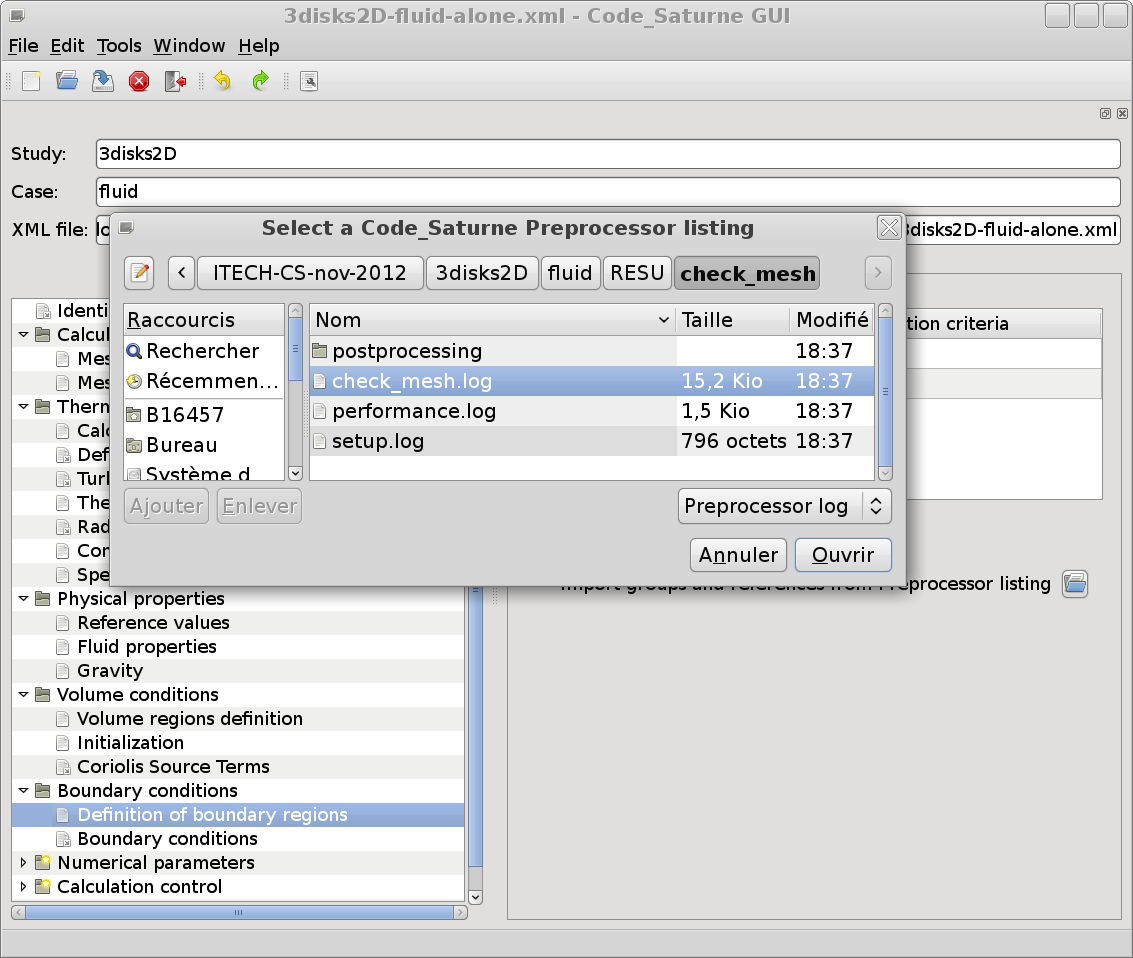
\includegraphics[width=9cm]{case6_fluid_V-7}
\caption{Load the check\_mesh.log file inside the \CS (GUI).}
\label{fig1_e5}
\end{center}
\end{figure}

%[4]
\newpage

\begin{figure}[h!]
\begin{center}
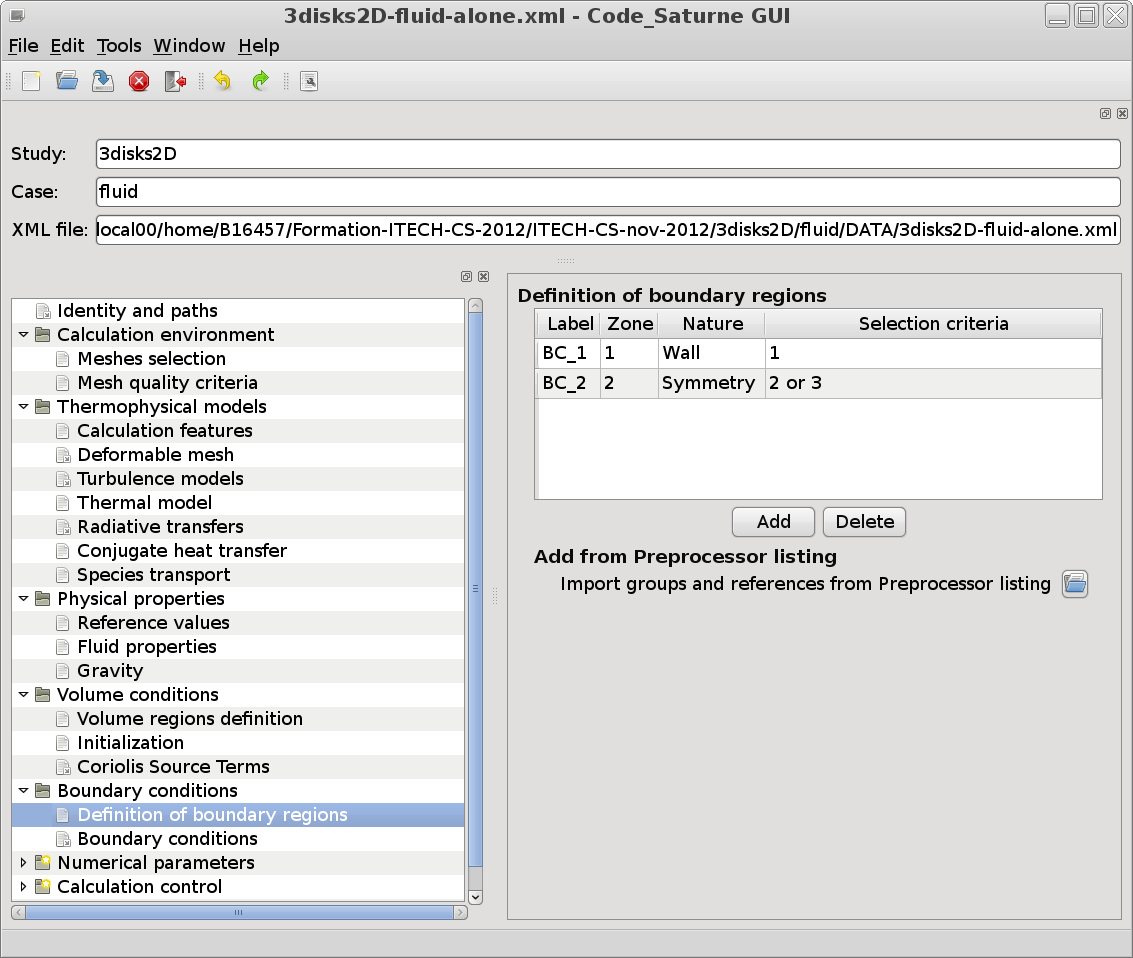
\includegraphics[width=9cm]{case6_fluid_V-8}
\caption{Loading the check\_mesh.log file automatically defines the boundary regions.}
\label{fig1_e5}
\end{center}
\end{figure}

\begin{figure}[h!]
\begin{center}
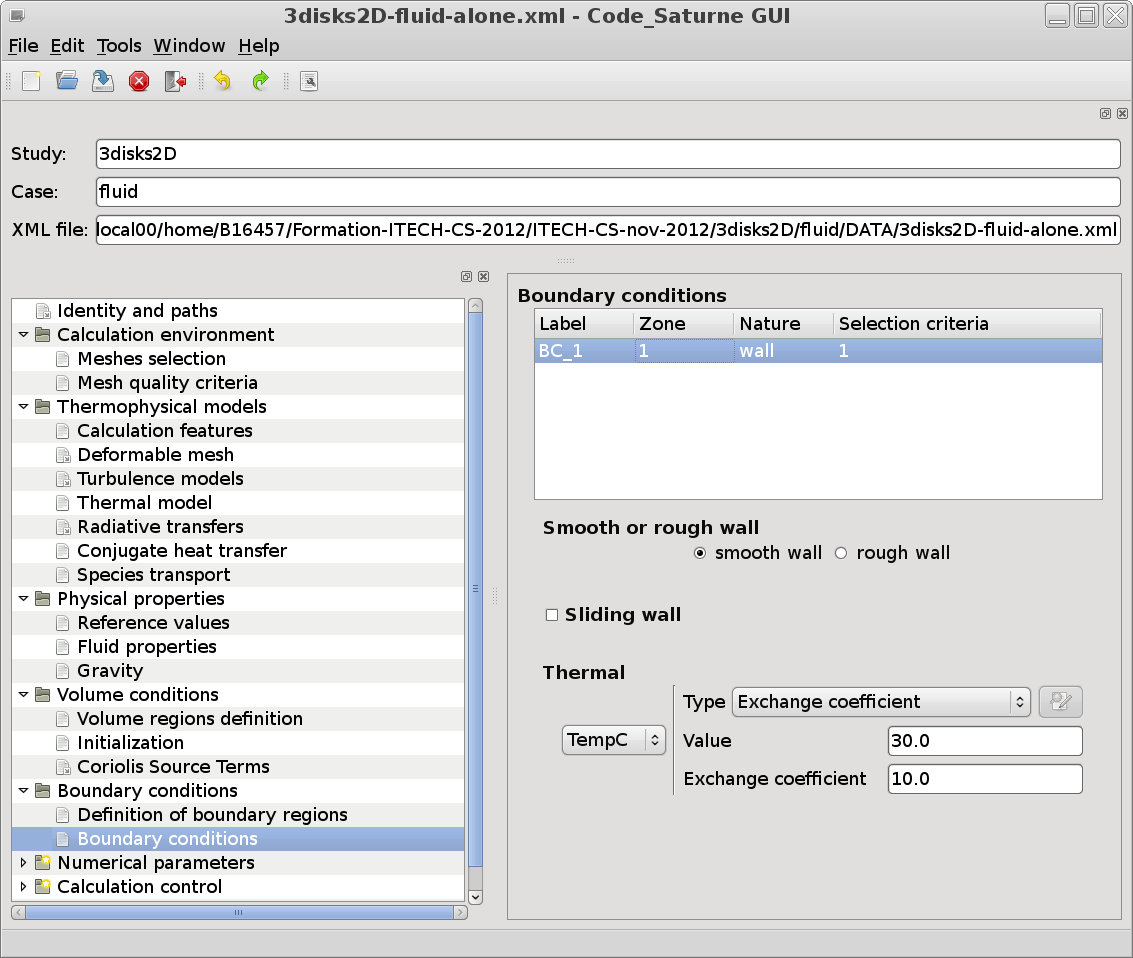
\includegraphics[width=9cm]{case6_fluid_V-9}
\caption{Define a thermal transfer condition as wall boundary condition with a extern wall
temperature T$_{\mbox{\scriptsize ext}} = 30 $\degresC ~and a exchange coefficient
q$_{\mbox{\scriptsize ext}} = 10$ ($W/m^2.K$).}
\label{fig1_e5}
\end{center}
\end{figure}

%[4]
\newpage

\begin{figure}[h!]
\begin{center}
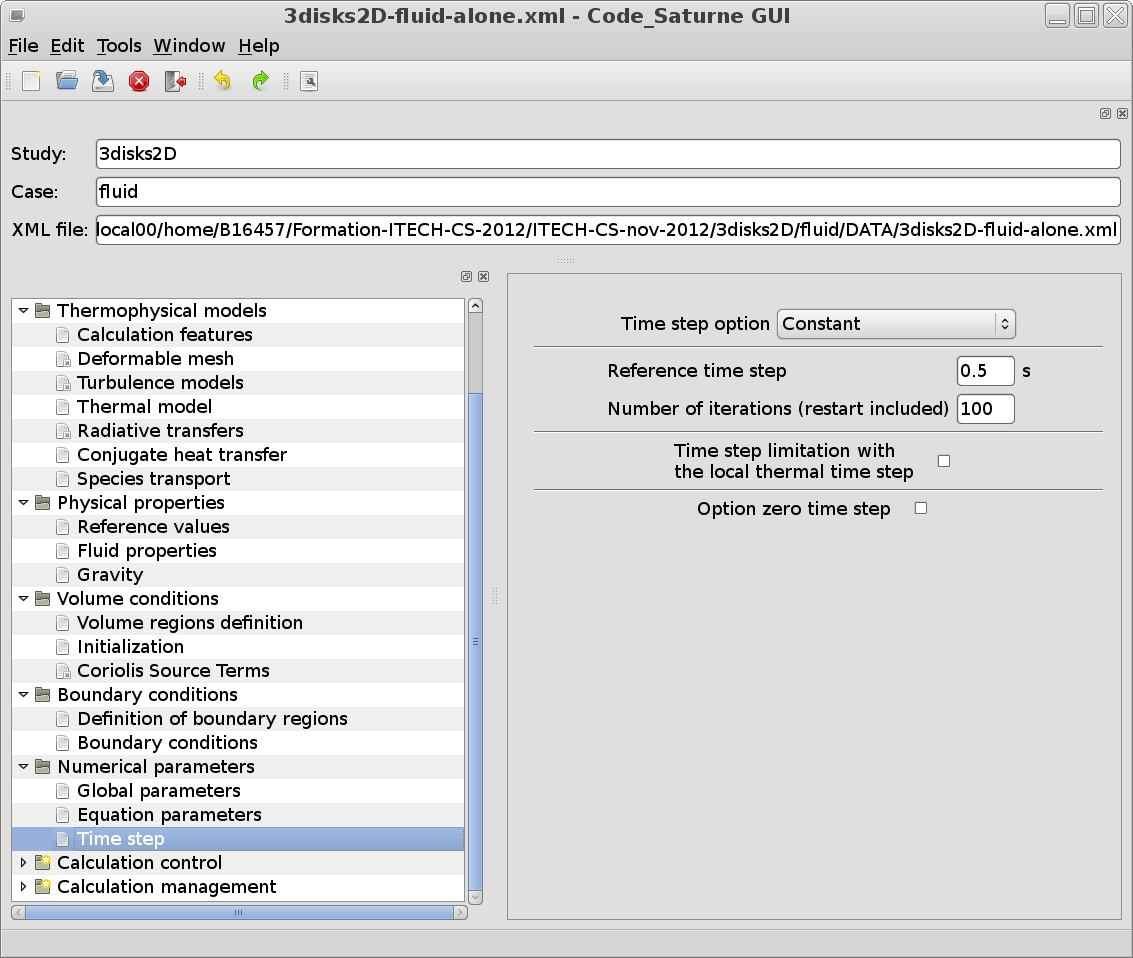
\includegraphics[width=9cm]{case6_fluid_V-10}
\caption{Define the iterations number and time step.}
\label{fig1_e5}
\end{center}
\end{figure}

\begin{figure}[h!]
\begin{center}
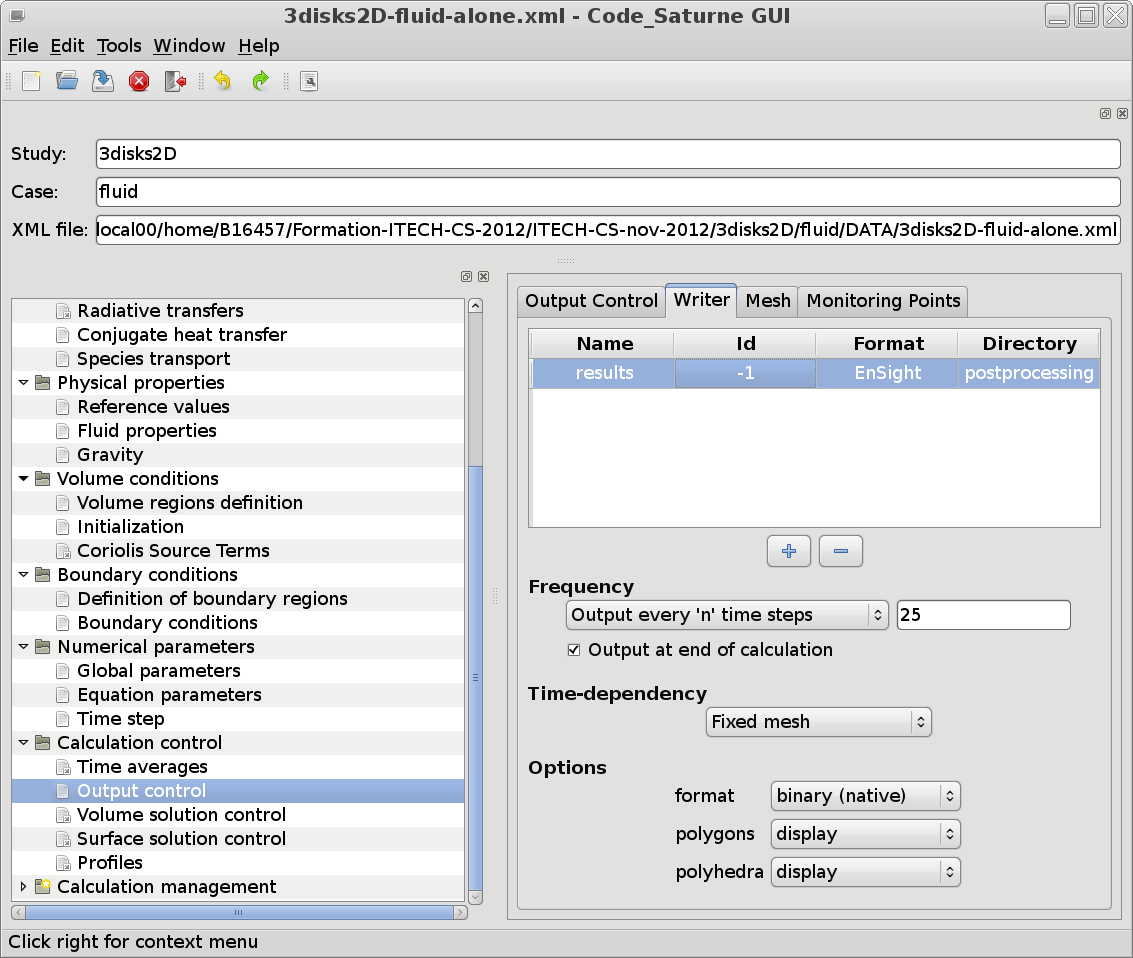
\includegraphics[width=9cm]{case6_fluid_V-11}
\caption{Define the writer and frequency output inside the \CS (GUI).}
\label{fig1_e5}
\end{center}
\end{figure}

%[5]
\newpage

\begin{figure}[h!]
\begin{center}
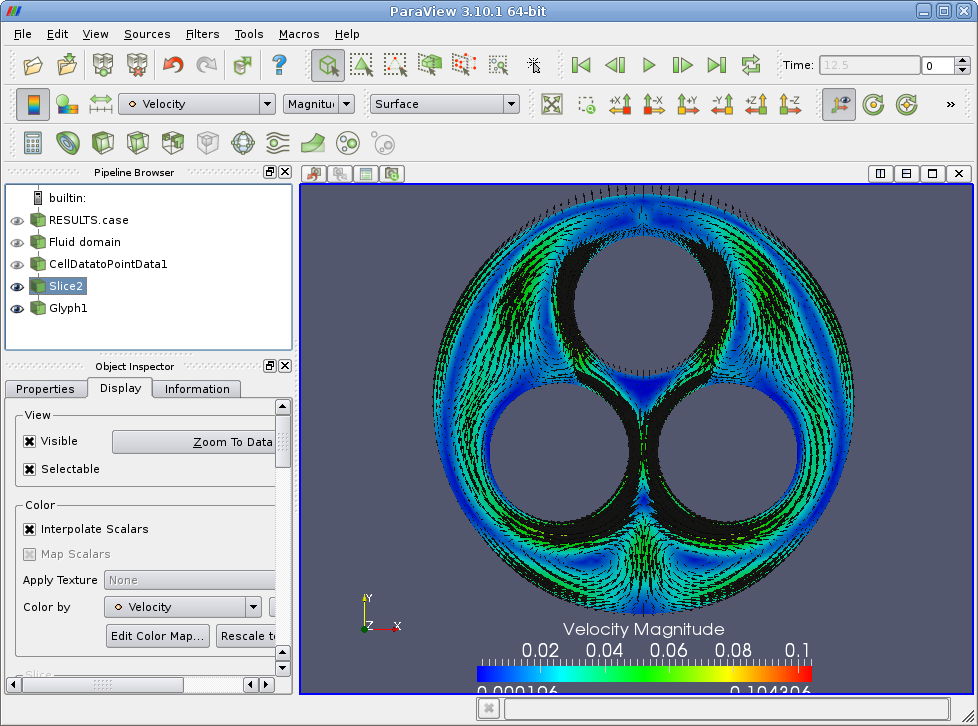
\includegraphics[width=12cm]{case6_visu_fluid-00}
\caption{Visualization of the 2D fluid velocity field}
\label{fig1_e5}
\end{center}
\end{figure}

\begin{figure}[h!]
\begin{center}
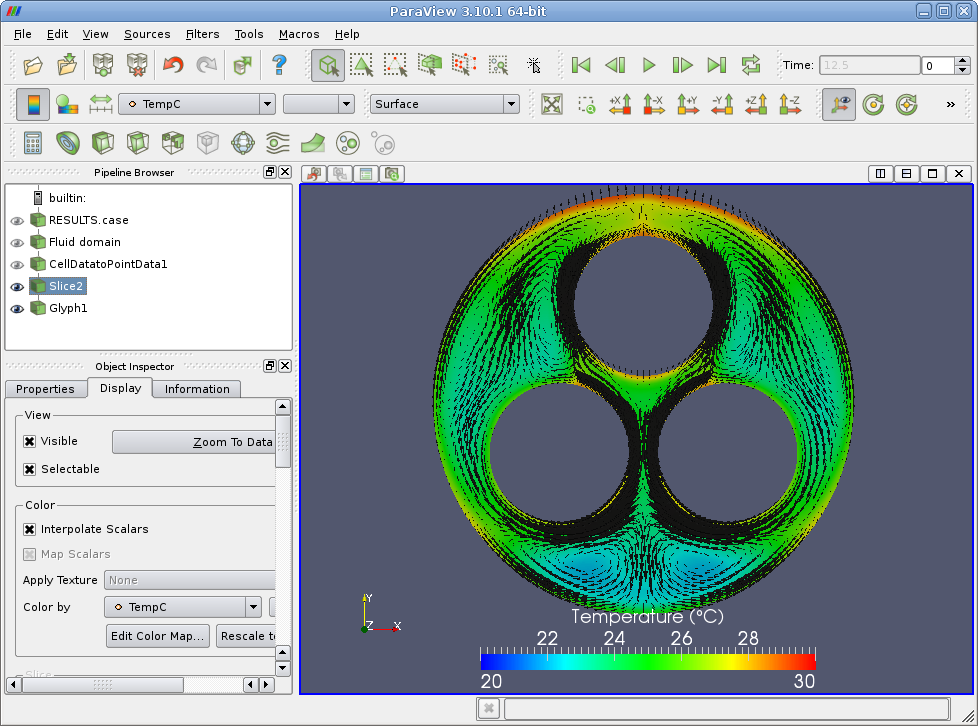
\includegraphics[width=12cm]{case6_visu_fluid-01}
\caption{Visualization of the 2D fluid temperature field}
\label{fig1_e5}
\end{center}
\end{figure}

%[6]
\newpage

\subsection{Launching the \CS-SYRTHES coupling computation}

The last modification to prepare the coupling computation are given below:\\
$\bullet$ {\bf Step 1}: activate the conjugate heat transfer in the \syrthes (Gui),       \\
$\bullet$ {\bf Step 2}: activate the conjugate heat transfer in the \CS (GUI),            \\
$\bullet$ {\bf Step 3}: give identical iterations number and time step for both codes,    \\
$\bullet$ {\bf Step 4}: check the \texttt{runcase\_coupling} script and launch it.        \\

\begin{figure}[h!]
\begin{center}
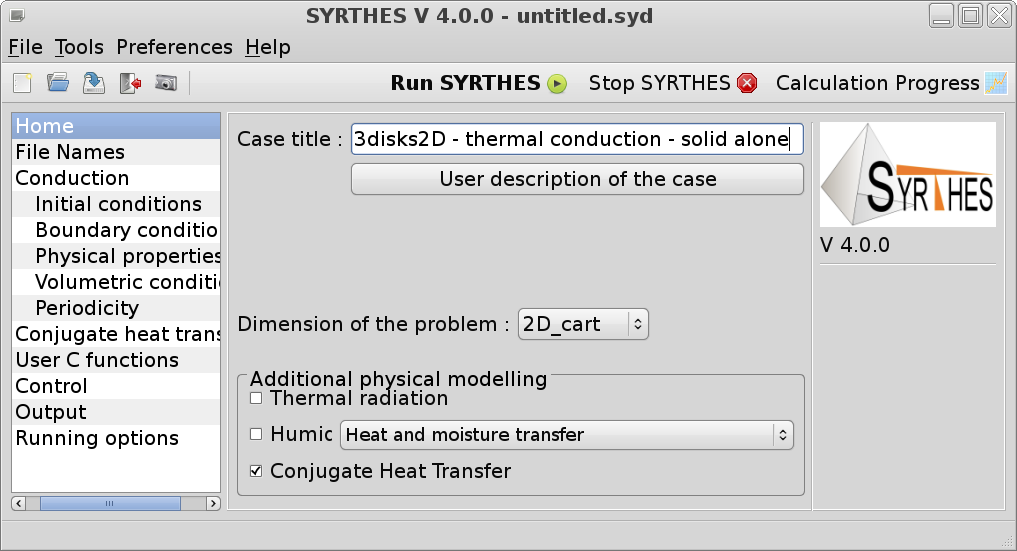
\includegraphics[width=12cm]{case6_solidcoupling_V-1}
\caption{Activate the conjugate heat transfer for the solid domain.}
\label{fig1_e5}
\end{center}
\end{figure}

\begin{figure}[h!]
\begin{center}
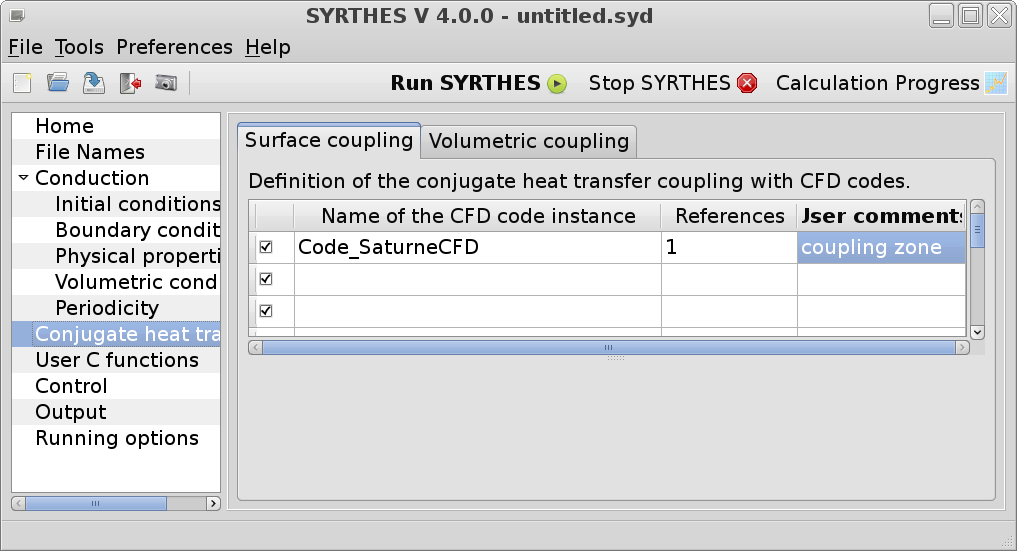
\includegraphics[width=12cm]{case6_solidcoupling_V-2}
\caption{Specify the reference zone for the coupling surfaces with \CS.}
\label{fig1_e5}
\end{center}
\end{figure}

%[1]
\newpage

\begin{figure}[h!]
\begin{center}
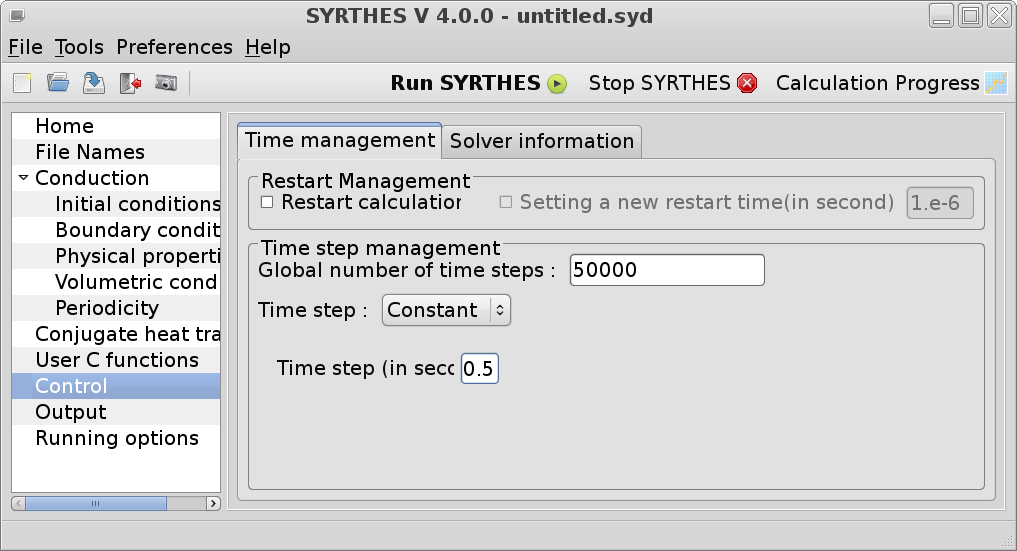
\includegraphics[width=12cm]{case6_solidcoupling_V-3}
\caption{Change the iterations number and time step for the solid domain.}
\label{fig1_e5}
\end{center}
\end{figure}

\begin{figure}[h!]
\begin{center}
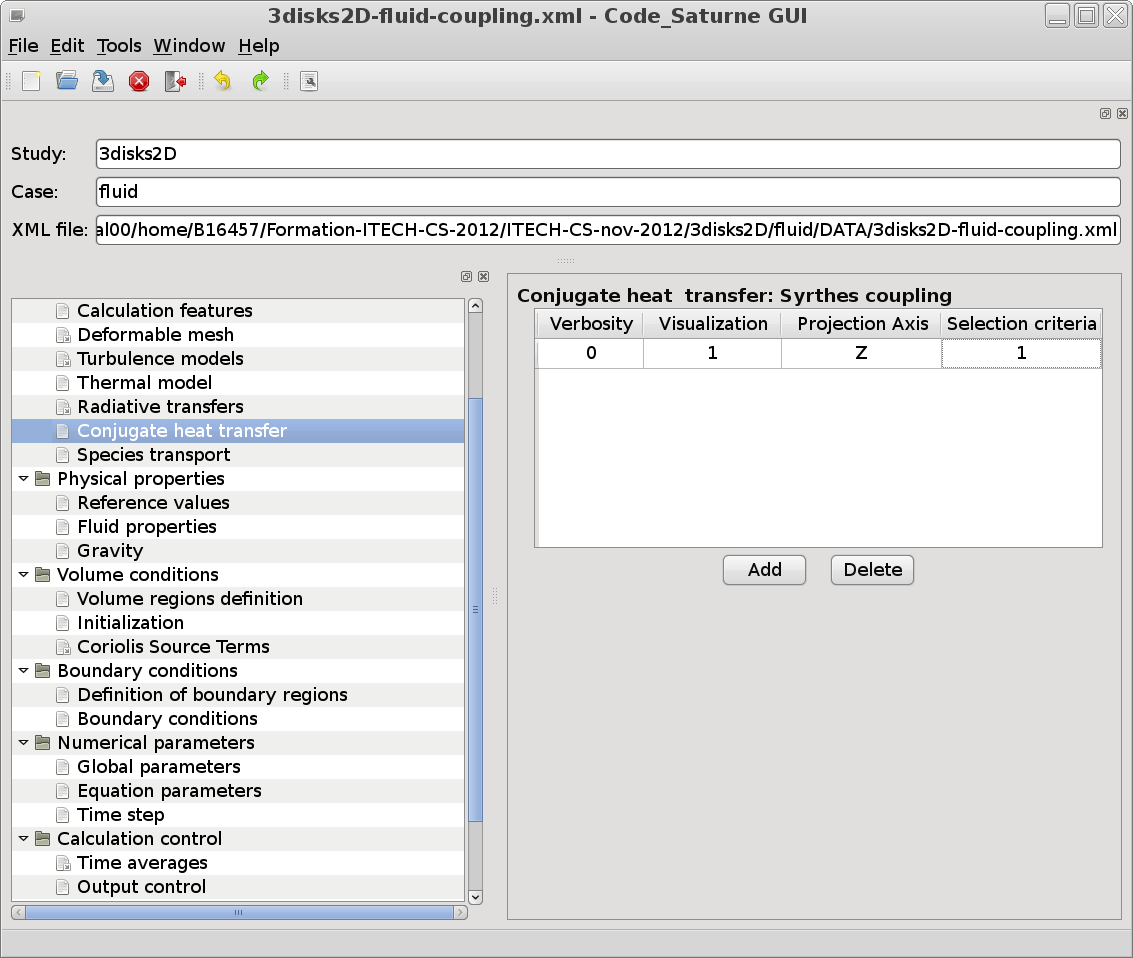
\includegraphics[width=12cm]{case6_fluidcoupling_V-1}
\caption{Activate the conjugate heat transfer for the fluid domain.}
\label{fig1_e5}
\end{center}
\end{figure}

%[2]
\newpage

\begin{figure}[h!]
\begin{center}
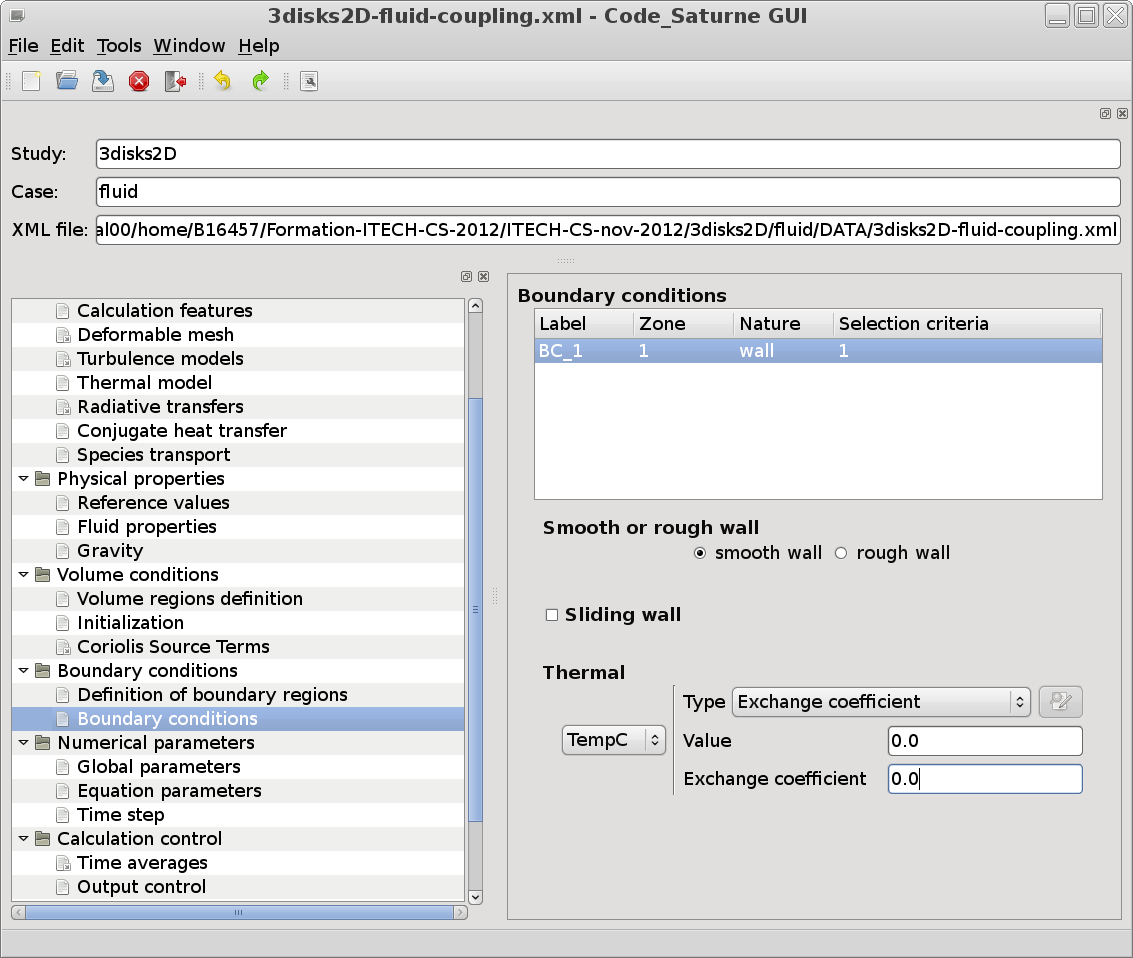
\includegraphics[width=9cm]{case6_fluidcoupling_V-2}
\caption{Change the boundary conditions for the wall temperature.}
\label{fig1_e5}
\end{center}
\end{figure}

\begin{figure}[h!]
\begin{center}
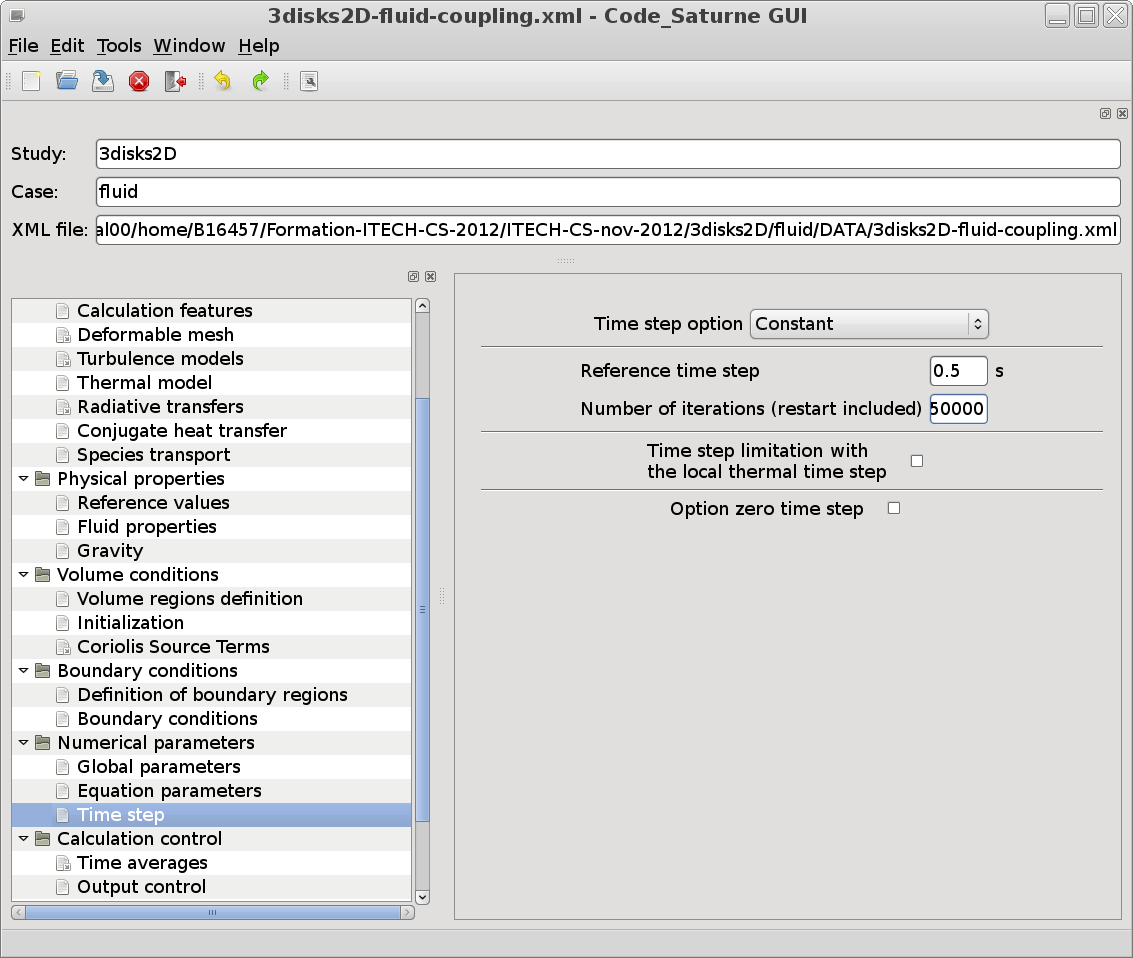
\includegraphics[width=9cm]{case6_fluidcoupling_V-3}
\caption{Change the iterations number and time step for the fluid computation.}
\label{fig1_e5}
\end{center}
\end{figure}

$\bullet$ {\bf Remark}: After having modified the data setting for the fluid
and solid domains to activate the conjugate heat transfer on both sides,
we just have to increase the iterations number and check the \texttt{runcase\_coupling} script.
\newpage
We just need to edit the \texttt{runcase\_coupling} script and give the name of your \syrthes
script saved in the \syrthes (Gui) as below: \\
\fbox{\begin{minipage}{\textwidth}\texttt{         \\
\$ vim runcase\_coupling                           \\
> domains = [                                      \\
>                                                  \\
>    {'solver': 'Code\_Saturne',                   \\
>     'domain': 'fluid',                           \\
>     'script': 'runcase',                         \\
>     'n\_procs\_weight': None,                    \\
>     {\color{blue}'n\_procs\_min': 4},            \\
>     {\color{blue}'n\_procs\_max': 4}}            \\
>                                                  \\
>    {'solver': 'SYRTHES',                         \\
>     'domain': 'solid',                           \\
>     'script': {\color{green}'solid-coupling.syd'},\\
>     'n\_procs\_weight': None,                    \\
>     {\color{blue}'n\_procs\_min': 2},            \\
>     {\color{blue}'n\_procs\_max': 2},            \\
>    \color{red}{'opt' : '-v ens'}}                \\
>                                                  \\
>    ]                                             \\
}\end{minipage} }

You just have to launch the \texttt{runcase\_coupling} present
in the study directory (named in our case \texttt{3disks2d})
and run the coupling computation, as follows:    \\
\fbox{\begin{minipage}{\textwidth}\texttt{         \\
\$ {\color{blue}runcase\_coupling}
}\end{minipage} }

$\bullet$ {\bf Remarks}: in the \texttt{runcase\_coupling}, you
can specify the processors number for each code (as this example
with 4 processors for \CS and 2 processors for \syrthes)
in parallel or just one processor for each code in sequential.

You can specify the ouput results format for \syrthes with an option
(\texttt{opt}) which takes the value \texttt{-v ens} for
a 3D fields output with a \ensight format or  \texttt{-v med} for
a 3D fields output with a \salome format).
%[3]
\newpage
